% This is samplepaper.tex, a sample chapter demonstrating the
% LLNCS macro package for Springer Computer Science proceedings;
% Version 2.20 of 2017/10/04
%
\documentclass[runningheads]{llncs}
\usepackage[hyphens]{url}
\usepackage{graphicx}
\usepackage{xcolor,colortbl}
\usepackage{mdframed}
\usepackage{multirow}
\usepackage{multicol}
\usepackage{comment}
\usepackage{amsmath}
\usepackage[utf8]{inputenc}
\usepackage[T1]{fontenc}
% Used for displaying a sample figure. If possible, figure files should
% be included in EPS format.
%
% If you use the hyperref package, please uncomment the following line
% to display URLs in blue roman font according to Springer's eBook style:

\mdfdefinestyle{RQFrame}{
 outerlinewidth=0pt,
 skipabove=0pt,
 skipbelow=0pt,
 innertopmargin=6pt,
 innerbottommargin=0pt,
 linewidth=0pt,
 topline=false,
 rightline=false,
 leftline=false,
 innerrightmargin=4pt,
 innerleftmargin=4pt}

\newcounter{RQCounter}
\newcommand{\RQ}[2]{
\refstepcounter{RQCounter} \label{#1}
\begin{mdframed}[style=RQFrame]\noindent
    \textbf{RQ}$_{\arabic{RQCounter}}$.~\emph{#2}
\end{mdframed}
}
\newcommand{\hr}[1]{\textbf{RQ}$_{\ref{#1}}$}
\definecolor{Gray}{gray}{0.9}
\newcommand{\mysubsec}[1]{\smallskip \emph{\textbf{#1.}}}



\usepackage{hyperref}
\renewcommand\UrlFont{\color{blue}\rmfamily}

\begin{document}

%
\title{Developing a hackathon approach to encourage cybersecurity learning}
%
%\titlerunning{Abbreviated paper title}
% If the paper title is too long for the running head, you can set
% an abbreviated paper title here
%
\titlerunning{Hackathon participation as a catalyst for cybersecurity learning}

%\author{Abasi-amefon O. Affia \and Alexander Nolte \and Raimundas Matulevi\v{c}ius }
%\institute{Institute of Computer Science, \\ University of Tartu, Tartu, Estonia,\\
%\email{amefon.affia@ut.ee, alexander.nolte@ut.ee, rma@ut.ee}
%}
%
\authorrunning{}
%\authorrunning{Affia et al.}
%
\maketitle              % typeset the header of the contribution
%
\begin{abstract}
Hackathons are increasingly popular across different domains in recent years including the security domain. Security research and development towards securing information systems% especially the internet of things (IoT) 
is on the increase due to the increased usage and possible applications. As such, there is a great need to train, spread awareness, and encourage people to explore the security of these information systems, and for that, hackathons might be a good approach.  This paper describes a hackathon approach applied at a hackathon event to encourage learning
in security for the participants. An action research study is used to introduce interventions that influence learning, this approach is analysed and the results discussed.
% findings
\keywords{Hackathons  \and Security \and Learning \and Action Research.}
\end{abstract}
%
%
%

\section{Introduction}
Technological advancements have led to the ubiquitous availability of data and shaped digital innovation \cite{davenport2013analytics}. Industry experts predict there will be 6 billion internet users by 2022 \cite{cybersecventures2019} and nearly 26 billion connected devices by 2020 \cite{hung2017gartner}. An important security measure for the success and growth of information systems is the level of knowledge and awareness among human users which build these systems and/or are a part of its network \cite{mahmoud2015internet}. It has been noted that there is a need for technical professionals important to guarantee for the rapid development of the Internet of Things even in the domain of security \cite{yu2010exploration}. 
%Education is one of the key enabling factors to achieving system security in smart industries \cite{tuptuk2018security}, 
However, there is widespread ignorance of likely threats and adversaries with end-users or administrators of these information systems. %In contribution to continuous research, development and innovation in IoT security, methods to improve cybersecurity learning as a contribution to already existing methods for IoT innovation is imperative. 
Cybercriminals are continually developing more advanced and scale able tools to access these user sensitive data. Already, more than 4.5 billion records were breached in the first half of 2018\footnote{\url{https://www.gemalto.com/press/Pages/Data-Breaches-Compromised-3-3-Billion-Records-in-First-Half-of-2018.aspx} (accessed at 11/03/2020)}. The security risks associated with information systems encompass people, process, objects, and data. So, securing these systems and raising awareness about how to securely use them is one of the great challenges of the coming years.  %Solving these challenges form a part of digital innovation and such innovations are as a result of collaborative processes in (interdisciplinary) teams rather than as the work of individuals\cite{steen2011benefits}.

Hackathons have been proposed as a great tool for teaching and spreading awareness and have been explored as an addition to the educational curricula \cite{abdullah2015stimulating,gama2018hackathons,sakhumuzi2017student,nandi2016hackathons}. This is because hackathons are where situated and collaborative learning take place and learning is one of the primary motivations for participants joining hackathons \cite{gama2018hackathons,briscoe2014digital,juell2014public}, where the acquisition of knowledge comes by practice and participants learning from one another and provided resources. Using the hackathon model, participants are encouraged to engage in intense collaboration to completing projects and produce outputs of new ideas, learning paths, technologies or prototypes over a defined period of time  \cite{nolte2018you,komssi2014hackathons}. 
%To accelerate the development of new service ideas and prototypes, innovation type contests, have become popular instruments \cite{bullinger2010innovation,hjalmarsson2012designing,soltani2014hackathon,juell2014public}. However, only a few of the service prototypes developed at innovation contests become viable digital services \cite{hjalmarsson2014beyond}. 
%However, few studies have addressed perceived learning in security based hackathons. 
Hackathons are a great tool that have been introduced to spread awareness and train users in various concepts of cybersecurity i.e  \cite{weiss2015teaching,kharchenko2016university,boopathi2015learning}. However, the intense nature of hackathons increases the significance of using special strategies or methods so that within the constraints, participants are still pushed to effective, collaborative and personalized learning outcomes \cite{kumalakov2018hackathon}, thereby achieving maximum learning output. So far, it is not clear which design aspects can foster awareness and cybersecurity learning.

Our study addresses this research gap by investigating methods and processes introduced to stimulate learning in security hackathons, thus answering the following research questions; 

%``\textit{How can one employ a hackathon to influence perceived learning in cybersecurity?}''. \\ This research question is investigated further to answer the following sub-questions;

\RQ{RQ1}{How can different interventions at a hackathon influence learning?}
\RQ{RQ2}{How can these interventions be improved?}
%\RQ{RQ3}{How do these introduced methods or processes influence learning at a hackathon?}

To answer these questions, we conducted an action research study of three teams at a cybersecurity hackathon. The methods and processes to stimulate learning were provided as interventions introduced during the hackathon process. We observed all teams and participants during the hackathon at set intervals during its early, mid, and later phases, administered surveys and conducted interviews at the end of the hackathon event.

Our results indicate ....

\section{Background}
Key domains that form the background of our work are discussed in this section including an overview of hackathons in security, the learning theory used in evaluation and related works.

\subsection{Overview of Hackathons in Security}
\begin{comment}
\begin{figure*}[h]
%\vspace{-15pt}
  \centering
  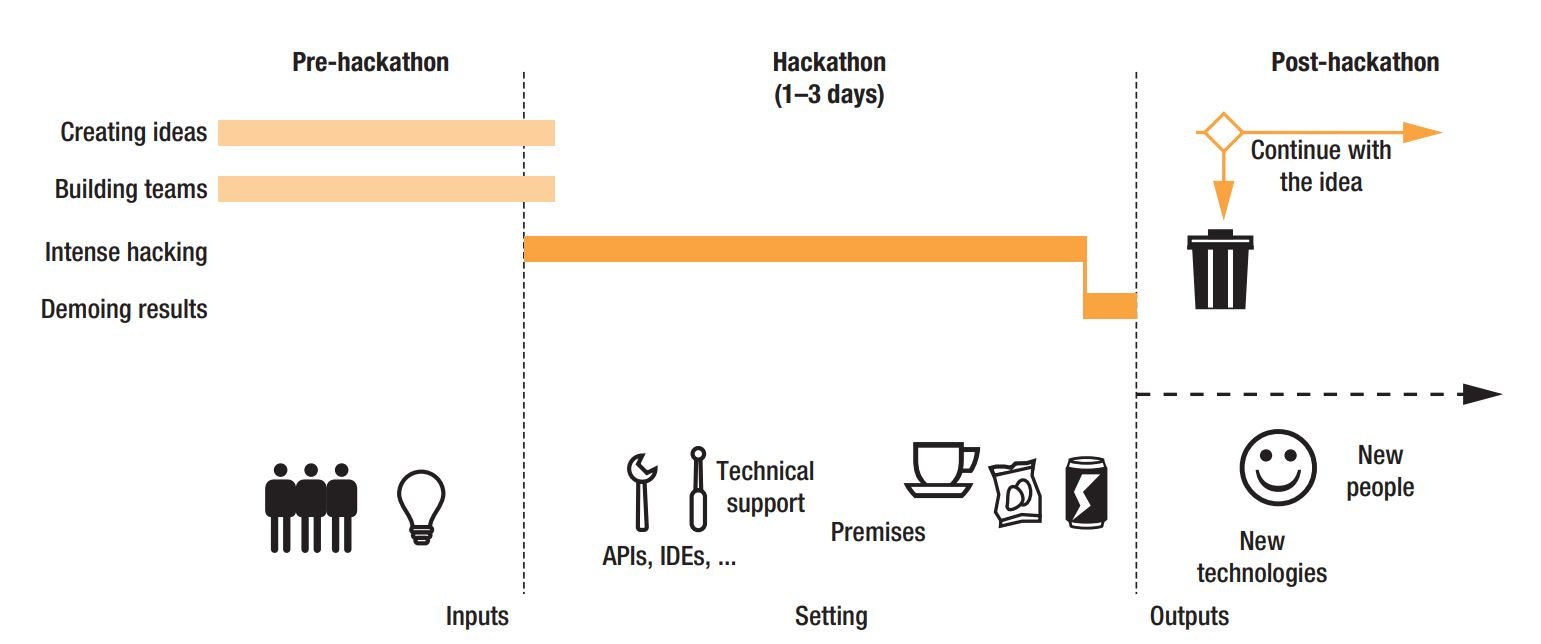
\includegraphics[width=0.75\linewidth]{hackprocess.JPG}
  \caption{Hackathon process adapted from \cite{komssi2014hackathons}} \label{Fig:hackprocess} 
 % \vspace{-20pt}
\end{figure*}
\end{comment}

Hackathons are intense, uninterrupted and \textit{time-bounded} events, typically of 2-5 days, during which people gather together and form \textit{collocated teams}, in attempts to complete a \textit{project} of interest\cite{nolte2018you,komssi2014hackathons}.

%Figure \ref{Fig:hackprocess} shows 
The typical hackathon process \cite{komssi2014hackathons} includes three stages -- pre-hackathon, hackathon, and post-hackathon phases. The pre-hackathon stage allows to better frame the problem to be solved or the hackathon event i.e. idea generation, team building. The hackathon stage (event) accelerates project ideas towards a prototype or other proof of concept, and the post-hackathon stage allows to develop a more robust product or service.

Hackathons in security cover the investigation of a topic, tool or technology within security and the developing of solutions with brainstorming and prototyping.
In security, hackathons have been widely introduced to facilitate training and awareness within the cybersecurity community to thereby improve and increase the cybersecurity workforce. In studies, saw that although hackathons in security are reported to be popular\footnote{\url{https://www.hackathon.com/theme/cybersecurity} (accessed at 11/03/2020)}, few of them have reported their findings academically. %However, from our findings, we could identify that hackathons in security are either in research, makeathon or gamification type formats. Research hackathons are where participants, usually students or researchers come together to discuss ongoing research, work on requirements, learn from each other about relevant technology and develop rapid prototypes. Makeathon type hackathons are a form of hackathons where the focus is on developing innovative hardware or software solutions to security issues. Lastly, gamification hackathons where a simulation environment is introduced e.g., cyber exercises and Capture-the-flag (CTFs) to test knowledge and practice of various computer security concepts and teams can compete in real time for prizes and bragging rights. 
As experts predict a global shortage of 2 million cybersecurity professionals by 2019 \cite{kauflin2017fast}, the hackathons in security attempts at bridging the gap between the fast growing need for cybersecurity professionals and the lack of appropriate security skills. Evaluations on the measure of cybersecurity learning during these hackathons is needed.

Paper  by \cite{kharchenko2016university}, presents a case study collection, some of which analyses the organisation of hackathons for cybersecurity development. In \cite{kharchenko2016university}, a hackathon is organised, targeted at learning cybersecurity features of embedded systems. Presentations on cyber security were made to provide cybersecurity knowledge and to discuss cybersecurity concepts. With knowledge gained, participants were divided into teams for a competition to solve a theoretical and practical problems per team, and results assessed by experts. Similarly, in \cite{starov2015hacking}, a case study defines hackathon organisation where students learn foundational and detailed knowledge in a special course, participate in training related to idea generation and prototype development, develop projects and then participate in competitions. In \cite{foley2018science}, a science hackathon is organised where researchers, using a transverse use-cases on shared CPS testbed platforms, explain ongoing research in securing cyber-physical systems (CPS), learn and teach each other about the technology, and develop prototypes. Learning experiences of the participants as well as the communicative ability of this hackathon about cybersecurity were discussed.

However, in these papers, design aspects that foster awareness and cybersecurity learning were not clearly evaluated. %include in each paper analysis.



\subsection{Design aspects of the hackathon for learning}
Learning approaches in a given environment determine if the participant learns at surface level, procedural deep level or deep level \cite{case2004between,marton1997approaches}. Surface learning approaches may not provide appropriate cybersecurity knowledge needed, and deep approaches may become an unrealistic goal within the given timeframe. Thus, an ideal learning approach for participants at a hackathon will be the procedural deep level suitable for learning through problem solving \cite{case2004between}. Here, enough knowledge about security can be gained to explore security research, contribute to the development of security solutions and/or compete in a security test within the given timeframe of the hackathon is achieved.

Designing hackathons that foster for learning in cybersecurity, involve careful goal planning and considerations because the designs and controls to the learning environment has great possibilities to influence learning. Strategic design decisions (SDD) and operational design decisions (ODD) are important to define the learning goals as well as other goals of the hackathon, and determine the workflows and processes that define specific settings at the hackathon \cite{kollwitz2019hack}. Dimensions of these design decisions are reviewed to discover those which specifically foster learning and explained in Table \ref{tab:designaspectforlearn}. 

%Discuss the selection of the interventions in general


\begin{table}[h]
\caption{Design aspects of the hackathon for learning}
    \label{tab:designaspectforlearn}
\begin{tabular}{|p{0.08\linewidth}|p{0.14\linewidth}|p{0.76\linewidth}|} \hline	
    & Dimension & Learning Characteristic  \\ \hline
	\multirow{2}{*}{\textbf{SDD}} & OI \newline integration & Involves the generation of ideas to solving a given challenge. Here, participants learn through discussions on the challenge subject domain, and by the development of the idea based on an understanding of the challenge. \\ \cline{2-3}
    & Value \newline proposition & Value proposition highlights the focus of the hackathon. This focus drives the theme and allows the participants to learn by accomplishing the challenge output. \\ \hline
	\multirow{2}{*}{\textbf{ODD}} & Incentives & Hackathons as team events and to encourage the value of cooperation and innovation within a given hackathon project and possibly, an encouragement to participate in learning.  \\ \cline{2-3}
	& Resources & Resources include other inputs provided to participants, before, during and/or after the hackathon that can encourage learning. \\ \cline{2-3} \hline
\end{tabular}
\end{table}



\section{Empirical Method}

The main aim of the research reported in this work was to investigate and understand how interventions within a hackathon can influence cybersecurity learning (\hr{RQ1}). To answer this question, we used an action research approach \cite{bhattacherjee2012social,kaplan1998innovation} to explore new forms of evaluating learning influence by set interventions. This approach is appropriate for this study because it provides guidelines to define actions to be introduced to a problem, to observe and study the introduction of these actions and analyse the results for future iterations. With action research, interventions are intentionally introduced to influence learning in cybersecurity, and then measures are taken to observe and understand the effects of the added actions. 

\subsection{Proposed Interventions to Learning} \label{Sec:interventions}
The proposed interventions include strategic and operational design decisions %\cite{kollwitz2019hack} 
that go into implementing the security hackathon. With the anatomy of the hackathon set, methods that provide learning opportunities in the hackathon were explored. Choosing interventions to introduce learning was guided by their suitability to the hackathon design. Following the action research design, we introduce and observe the effects of interventions in cybersecurity learning (\hr{RQ1}). We then analyse the effects of the interventions to suggest possible improvements to these actions(\hr{RQ2}).

%Elaborate on how these interventions are designed for this hackathon

\textbf{Idea generation} as an intervention provides the opportunity to generate ideas addressing security issues. This is to be provided to introduce the participants to the process of proper idea preparation and maturing and as a result, kick-start the hackathon process.  Encouraging idea generation especially before the hackathon event has the advantage that participants/teams can be more prepared, hence more efficient at the hackathon event. During idea generation, ideas are gathered in order to generate a pool of ideas where one or more ideas are selected based on the participants’ interests and/or skills \cite{bohmer2015open}. Ideas selected are further refined to ensure it aligns with the theme of the hackathon and holds value in solving real security issues. In Pe-Than et al. \cite{pe2018designing}, it is observed that winning teams are characterised by fairly extensive idea preparation. Idea generation is also an important factor in building a team of people with shared interest.
The learning objective from this intervention is that; (1) Participants should have an understanding of current security issues, (2) Participants should be able to propose ideas based on the knowledge gained, to address these security problems, (3) Participants should be able to communicate the impact that the security knowledge gained has on the development of the proposed solution. 

The introduction of \textbf{security talks} at the hackathon is done to provide context to the hackathon goal discuss the basics of security within the current advances in information systems with its existing security issues. Talks covered top security trends in IoT, security risks in IoT applications, and security risk management. These discussions are intended to introduce participants new to the field, to security and encourage other participants to learn more about security techniques and concepts. It allows participants produce better ideas generated with more concrete knowledge of the issues in security. The learning objective from this intervention is that; (1) Participants should remember basic security concepts learnt from the security talks, (2) Participants should be able to understand existing security issues and its impact.

Another intervention proposed is the \textbf{mentor feedback process}, to provide experience and insights to guide projects especially in scoping, given the limited time frame \cite{lara2016hackathons}. The mentor participation and assignment were organised in two ways, (a) during set checkpoint sessions, and (b) by need-based special assignment -- where teams with special challenges are assigned mentors that will help resolve these challenges. In the checkpoint sessions, participants are able to give short technical briefings or pitches about their ideas and product executions. This enables the teams to learn more about other teams process to solving tasks and gain some knowledge that will help accomplish their tasks. This is to be done in such a way that each group received sufficient participation of mentors. The learning objective from this intervention is that; (1) Participants should be able to incorporate mentor feedback to security solution, (2) Participant should be able to communicate the process of building the security solution as a result of knowledge gained.

Although participation in the hackathon is voluntary, \textbf{competition type design} features and incentives can shape participation \cite{grimes2008robotics}. A competition style hackathon was introduced as an incentive to teams to put more effort in their projects, with an aim to generate more unique solutions. Strategic competition prizes sets the goal for participants and provides the opportunity for further development in the form of providing additional resources post-hackathon including  startup incubator programs or the opportunity to pitch the idea to a top executive. These prizes were decided to be more strategic as opposed to cash because they present opportunities for continued development of winning ideas. The learning objective from this intervention is that; (1) Participants should be able to apply the security knowledge gained to create a unique security prototype within the given time frame.

%Interventions were proposed to enable the participants engage in one or more subcategories in the bloom's taxonomy. \subsection{Evaluation of Design aspects}\label{sec:blooms}
We also evaluate the effect of design aspects introduced and the learning objectives of the participants of the hackathon. We assess the learning objectives and knowledge gained by the participants using Bloom's Taxonomy, and the effect of the introduced design aspects in learning is analysed based on data collected about the hackathon event.

Bloom's Taxonomy describes levels of learning where categories of Remember, Understand, Apply, Analyze, Evaluate, and Create form the cognitive learning process dimension that participates in knowledge dimensions \cite{bloom1956taxonomy,krathwohl2009taxonomy}.
\begin{itemize}
    \item \textbf{Remember} includes the retrieving, recognizing, and recalling relevant knowledge provided by the design aspects from memory.
    \item \textbf{Understand} constructs meaning from oral, written, and graphic messages through interpreting, exemplifying, classifying, summarizing, inferring, comparing, and explaining.
    \item \textbf{Apply} uses a given procedure through executing or implementing.
    \item \textbf{Analyze} separates knowledge or concepts into constituent parts, determining how the parts relate to one another and an overall purpose.
    \item \textbf{Evaluate} makes judgments based on criteria and standards through checking and critiquing.
    \item \textbf{Create} puts elements together to form a new pattern or structure.
\end{itemize}
In studies, the taxonomy has been used, especially in computer science fields, to assess learning outcomes and objectives that formulate how an educative process \cite{starr2008bloom,thompson2008bloom} improves students knowledge. Using bloom's, we can discern if the participants are familiar with security concepts presented at the hackathon, and can form relationships between the essential elements of security to develop a security idea. We can also discern how this knowledge was used as a baseline to carry out the intended project and, as a result, create a security prototype.

As studies do not specify which design aspects introduced in the hackathon serve to encourage learning, the connection between the levels of learning and the introduced design aspects will give us insight into what design aspects were instrumental to learning. This insight will enable us to build on such design aspects in the future, to advance security awareness and reduce the cybersecurity knowledge and skill gap.

%The taxonomy to analyse the assessable learning outcomes of each introduced design aspect. We can discern if the participants are familiar with basic security concepts, can form relationships between the essential elements of security, and use this knowledge as a baseline to develop a method of carrying out the intended project and, as a result, create a security prototype.

%The knowledge dimension follows Bloom's knowledge categories. These allow us to assess if the participants are familiar with basic security concepts, are able to form relationships between the basic elements of security and use this knowledge as a baseline to form a method of carrying out the intended project and as a result create a security prototype. The cognitive process dimension allow us to assess knowledge gained through each step of its process.

\subsection{Setting and procedure}
The hackathon we studied was a 48 hour event organised with the main aim to expose participants in cybersecurity problems, with a view to finding solutions to these recurring problems and challenges. % and to come up with innovative approaches to security in general and IoT security. 
Solutions expected range from security awareness to security software/hardware prototypes. 
\begin{figure*}[h]
%\vspace{-15pt}
  \centering
  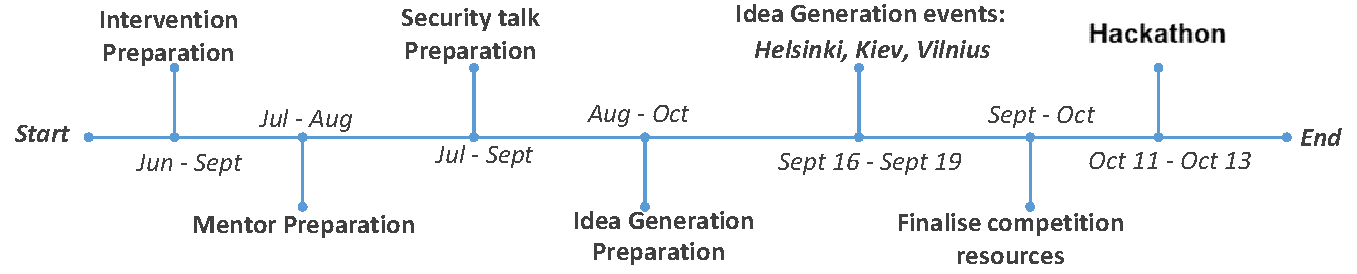
\includegraphics[width=\linewidth]{timelinehack.pdf}
  \caption{Preparation activities and data collection before, during and after the hackathon event} \label{Fig:timeline} 
 % \vspace{-20pt}
\end{figure*}
Preparations for the hackathon event began 5 months prior to the event. Fig \ref{Fig:timeline} shows the timeline of the hackathon process including preparation and data collection activities before during and after the hackathon event. The proposed hackathon included a pre-hackathon, hackathon and post-hackathon phase \cite{komssi2014hackathons}. The pre-hackathon phase will be treated as a separate event from the hackathon phase. This event is mainly to boost idea generation, security knowledge exchange, and bring people together from different fields to generate ideas that aim at tackling issues in cybersecurity. Pre-hackathon events were organised from 16th till 19th September, 2019. These events started out with a session to discuss on the different challenges and problems in the field, followed by a talk on how to effectively communicate ideas. After the first round of idea generation, we provided exercises that help participants think deeply and elaborate on these ideas. Sessions were also conducted with the help of skilled mentors, providing feedback on each proposed idea and there was a great opportunity to mature ideas that can be turned into innovative prototypes. These idea garages were conducted in three cities -- Helsinki, Vilnius, and Kiev -- serving to spark interest in the hackathon and raise awareness of its capabilities. A total of 17 ideas were generated, and 11 of those ideas were developed and pitched at the idea garage. 

The hackathon itself started with a short introduction by the hackathon organizers and mentors and an introduction to the domain by a short talk on security. Participants were able to listen to the security talks posed about security issues and develop ideas to solve these problems. These ideas were pitched to mentors and fellow participants, highlighting how the proposed product will solve cybersecurity issues. The mentors asked questions and provided feedback on the proposed ideas to develop them further. This led to a total of 17 ideas for further refinement. An idea from the idea  garage pre-hackathon event was presented during the hackathon event. Mentors facilitated a documentation of all ideas and provided these to the participant for possible team formation. Once the idea generation sessions were completed, idea selection commenced. Ideas selected was due to the availability of team members at that moment or interested participants for the ideas. 
Team formation exercise led to a healthy size of team members per selected idea. Once team formation for selected ideas was completed, team work on the selected project idea commenced. Out of 17 ideas pitched, 10 ideas were selected to form a suitable team. Checkpoints during the hackathons enabled teams provide updates on the solutions to the proposed ideas. Two checkpoints were set and mentors were available to provide expert guidance and feedback concerning the solution and team progress. A special security talk was also provided on security risk management, to provide the participants with more security considerations when building their solutions. 
All teams presented their solutions and prototypes at the end of the hackathon for evaluation by judges. This presentation was live streamed to all interested community members. After evaluation, the winners were selected and teams could win different prizes. 

\subsection{Data collection}
We collected data for this study from different sources including planning documents, data by observation, survey, and post-hackathon interviews (c.f. Fig. \ref{Fig:timeline} for an overview of the time-line).  We will expand on how data collected from these data sources contribute to answering research question \hr{RQ2}. %and \hr{RQ3}.

Before participating in the hackathon, participants filled out an online registration form containing questions about demographic background and skills. %possessed. 
These answers provided information relevant to aid team formation, security presentations to be delivered, and mentor compilation for the hackathon.

%To observe the participants activities and behaviour one researcher was assigned to the 3 teams analysed. 
We moved between the teams during the hackathon event to observe the participants activities and behaviour.
The observation method included the monitoring at intervals and recording the behaviours of the participants in relation to the interventions to influence learning in cybersecurity.  %Prior to the hackathon, an observation scheme was developed to record how the participants interacted or reacted to the interventions introduced influence learning (\hr{RQ1}).  

as well as other factors that may contribute to understanding the learning experience of the participants such as team work, team process, or leadership influence. The perceived satisfaction of participants to the project and security was also noted.  We did not observe the teams throughout the duration of the hackathon as we perceived the early, mid and late phases of the hackathon to be important. The outcome of individual talks with participants were recorded as well.

After the hackathon event, post-hackathon surveys were supplied to the participants. The voluntary survey covered participants motivation and preparation for the hackathon, team demographics and process, learning experience based on the interventions, and satisfaction with the experience on a 5-point likert response scale. A total of 13 responses (from 7 projects) were collected from the survey. Sample questions include; 
\begin{enumerate}
    \item To what extent was your decision to participate in the cybersecurity hackathon motivated by:[\textit{options list}]
    \item How did you work together on your project during the hackathon? [\textit{options list}]
    \item To what extend do you agree with the following statements about your cybersecurity learning experience at the hackathon? [\textit{[options list]: Talking with my mentors helped me learn more about cybersecurity}]
    \item Please indicate your level of agreement with the following statements related to the satisfaction with your learning experience: [\textit{options list}]
\end{enumerate}


Post-hackathon interviews were then conducted with invited participants to discuss the preparation process for the hackathon, what was learned, and the project solution worked on. The interviews are to last about 30 minutes. These post-hackathon interviews are conducted and analyzed for participants to provide better comprehension of perceived individual and team learning experiences.

\begin{enumerate}
    \item How was the hackathon from your perspective in the form of: What did you do after you arrived? How did you see the event play out? 
    \item Did you attend the pre-event? What idea did you come up with? How else did you prepare for this hackathon?
    \item What were the outcomes as a result to learning? [mentors, security talks, team members, working on project]
    \item How do you perceive the outcome of the hackathon? Were you satisfied? How did you see your teamwork? 
    \item What security issues did your project address? What security considerations were placed on the [process of creation of product, final outcome of project].
    \item Did you discover anything new as regards security during the hackathon? How did you discover this?
    \item What about continuity of your project? Have you use anything learned during the hackathon already? or Are you panning to use it in the future? 
    \item Do you still use any security knowledge gained during the hackathon?
\end{enumerate}

\subsection{Analysis procedure}
The analysis procedure started by analyzing interview recordings, survey results, observation notes and planning documents. The interviews and observation served as our main source of information with planning documents providing additional context. We used the surveys as additional qualitative data complementing the interview recordings.

We focused on the team as our unit of analysis, analysing how the participants in a team responded to the interventions of idea generation, security talks at the event, mentor feedback process and the competition design type. Some interesting parts of the hackathon i.e., satisfaction with the final product, team demographics i.e (size, skill diversity, familiarity, leadership) were included where they may have affected the learning experience.

%Most of the data were collected in a straight-forward manner from the surveys, however, 
Data concerning the team demographics i.e., skill diversity was derived by calculating the similarity of perceived team skills and then revert the result by subtracting it from one. %To arrive at a team level measure, we create the union of all perceived skills of all team members. Using this union as a basis we then calculate the overlap of each individual team member with the overall perceived skills of the entire team and divide the result of this calculation by the size of the union of all perceived team skills. Adding up all scores for each team, we then divide the results by the number of team members to arrive at a normalized team measure.
%\begin{center}
%    $1 - (\sum_{k = 1}^{n}(\text{\#skills}_{k} \text{/ \#all skills}) \text{ / n})$
%\end{center}
Data from each relevant survey question is mapped to its corresponding point for analysis. This qualitative data will complement further analysis done using the observation and interview. For this mapping we followed a strategy \cite{braun2006using} by creating and applying initial codes to the interviews based on our research questions and interesting points that could also help answer research questions. Findings for each team were then compared to assess the perceived learning of one team over another.

In assessing the perceived learning, we used blooms taxonomy\cite{bloom1956taxonomy,krathwohl2009taxonomy} to analyse the processes by which the participants encountered and worked with knowledge provided through the interventions (see table \ref{tab:bloomsubcategories}. Each category represents the combination of the appropriate knowledge level to learning process encountered by the participant during the execution of the project idea at the hackathon event.

\section{Findings}
This section outlines the journeys of each selected team, the influence of each learning intervention on each team, and the differences between teams relation to their learning process with the introduced interventions.
%\subsection{Description}
The learning experiences within the team are gathered from data sources of observation, survey and  post-hackathon interviews. 
\begin{table}[h]
    \caption{ Statistically significant questions and responses from survey for learning}
    \label{tab:teambinter}
    %\centering
    \begin{tabular}{|p{0.22\linewidth}|p{0.42\linewidth}|p{0.1\linewidth}|p{0.1\linewidth}|p{0.1\linewidth}|}\hline
	Intervention & Significant \newline Survey Question (see Appendix) &  Team A & Team B & Team C \\ \hline
	Idea generation & Q3, Q13 & $\emptyset$ & 2.25 & 2.5  \\ \hline
	Security Talks  & Q13 &  4 & 3 & 3.67   \\ \hline
	Mentor Feedback  & Q13 &  3.5 & 3 & 3.33 \\ \hline
	Competition style \newline (Final Product) & Q4, Q13, Q14, Q15 & 3.3 & 3.3 & 2.7   \\ \hline
	\multirow{8}{*}{**Team properties} & size (Q5) & 6 & 6 & 5  \\\cline{2-5}
	%& skills (Q1**, Q3) & 0.5 , 1 & 0.5,2.5 & $\emptyset$, 1  \\ \hline
	& team familiarity (Q9) & 1.125 & 4 & 1  \\ \cline{2-5}
	& motivation (Q2) & 3 & 3.92 & 2.56  \\ \cline{2-5}
	& preparation (Q4) & 1.25 & 2.75 & 1.33  \\ \cline{2-5}
	& leadership (Q7) & yes & yes & yes  \\ \cline{2-5}
	& skill diversity (Q8) & 0.6 & 0.7 & 0.4  \\ \cline{2-5}
	& collaboration process (Q10,Q11) & 3.81 & 4.56 & 4.125  \\ \cline{2-5}
	& satisfaction(Q12, Q13) & 4, 3.813 & 2.9, 2.8 & 3.5, 3.2  \\ \hline
    \end{tabular}
    %*Partial evaluation as Q3 did not apply \\
    *Not interventions but these team properties that were found interesting in analysis.
\end{table}
\subsection{Team A}
The leader of Team A (P01) proposed the idea for the project carried out by the team because he ``\textit{remembered a security problem from studies during the Idea pitching session''} (P01) of the hackathon. This idea was refined by mentors during this pitching session to provide the initial description of the team idea, where they intended to create tool for enterprises to visualize security aspects. The team was formed at the team formation session after a quick idea generation session at the beginning of the hackathon event. At the start of the team formation session, ``\textit{team formation was difficult as there were not enough members at first}'' (P01), however, the team grew into a 6-member team with skill diversity rated at (\textit{0.6}) but with minimal familiarity with each other ($\overline{x} = 1.125$). \textit{``Ideation continued during the hackathon because the idea was not properly prepared''}, (P01) but with a number of discussions within the team and with mentors, the idea was refined to ``\textit{be targeted at company risk management team to help visualise and communicate security risk scenarios to upper management}''. Even with the difficulties of idea generation at the hackathon event, P01 highlighted that ``\textit{other than these difficulties, working on the hackathon was an educating experience about risk management and what is missing in the cybersecurity field}'' (P01). There was a moderate to low agreement on the idea generation phase ($\overline{x} = 2$) helping the team to learn more about cybersecurity. Security talks were also made in the pre-hackathon and hackathon event which helped the team learn more about cybersecurity ($\overline{x} = 4$) and the team showed an understanding of the security domain in moving forward with the project. 

After the initial difficulties in idea generation and refinement, there was great ``\textit{support by experienced team members to complete tasks}'' (P01) for the project. The team also incorporated lessons learnt from the hackathon event security talk in creating the final prototype. The team leader (P01), was involved in \textit{``holding everything together, monitoring and identifying the needs of each team members for completing tasks''} as well as decisions on the direction of the project. These responsibilities of the team lead were supported by mentors where necessary in order to adjust scoping of the project. ``\textit{Teamwork was growing and everybody was eager to work and contribute in way they could}'' (P01) and ``\textit{some team members had no prior experience to security, but they tried to learn and contribute}'' (P01). P01 thus reported that, ``\textit{they went definitely beyond their current skills}''. At checkpoints in the hackathon event, the team leader P01, presented updates to the mentors about the project progress, getting feedback from mentors about moving forward to prototype stage. Talking and interacting with mentors was reported to help the team learn more about cybersecurity ($\overline{x} = 3.5$).

Nearing the end of the hackathon event, the project pitches were conducted and following competition judging criteria, Team A's prototype was evaluated. Although team A did not win a prize at the event, there was reportedly, a moderate learning experience from building the final product ($\overline{x} = 3.3$) and an agreement on the satisfaction level from the event ($\overline{x} = 3.9$), with special comments about the \textit{``great event setup and mentoring''} (P01) and how \textit{``nicely organized''} (P02) the event was. %(Q12, Q13)
Other forms of learning also occurred by \textit{``practicing theory taught in class''} (P01) when handling the project, and the hackathon was beneficial as it has \textit{``strengthened [my] knowledge to provide better service at my work place''} (P01). However, P01 expressed that there will be no continuation in the project because it was \textit{``not quite sure, the market value for this type of project''} (P01), having less intent to continue with project as opposed to another team member P02.


\subsection{Team B}
P03 \textit{``got alot of support to [my] idea during the idea generation phase''} (P03) at the pre-hack event and \textit{``already had a team idea before the hackathon''} (P04). There was a moderate familiarity with hackathons within the team ($\overline{x} = 2.5$), however there was some familiarity between members of the team socially ($\overline{x} = 4$). The idea developed was to \textit{``make data security more desirable for startups and give them a badge''} (P03), thereby tackling the security awareness in startups issue. This idea was presented during the idea pitching session of the hackathon event where there was not much refinement to be done by mentors. Team formation was easy as P03, the idea visionary, \textit{``was familiar with most of the team because [we] studied together at the university''} (P03) and finally, forming a 6-member team with skill diversity rated at (\textit{0.7}). With idea preparation completed, the team went right into working on tasks to complete the project. Proper idea preparation allowed more time for working on the project tasks. 

In handling the tasks, Team B showed high collaboration ($\overline{x} = 4.6$) and team process ($\overline{x} = 4.5$). This collaboration was aided as there was a \textit{``blackboard equipment for documentation of the teams process and ideas, allowing [us] to see the big picture''} (P03). Mentor feedback was helpful as the checkpoints provided \textit{``an opportunity for [us] to explain our work progress''} (P04) and between checkpoints, \textit{``mentors visited to provide guidance on completing tasks''} (P04). Mentors specifically provided feedback on the scoping of the project and refinement of project content to define the life-cycle of different startups and the security implementations needed for each stage of the life-cycle as well as the business aspects. However, P04 highlighted that there were \textit{``too many mentors and once they changed each time [we] had to introduce our project from the very beginning''} (P04). The security talks at the hackathon event was instrumental as the team \textit{``tried to gather all sorts of information on how to secure systems, and gained new knowledge''} (P04). There was a moderate agreement on the security talks and mentor feedback($\overline{x} = 3$), and a moderate to low agreement on the idea generation($\overline{x} = 2.25$) helping the team to learn more about cybersecurity. 

Towards the end of the hackathon event, Team B pitched their project and presented the prototype for evaluation. Team B won a prize for unique product developed and its perceived usefulness to the security community. Interestingly, there was a moderate satisfaction with the outcome of the project ($\overline{x} = 2.9$). The bulk of the learning for team B seemed to be as a result of accomplishing the task of building security content, however, there was a moderate perceived learning experience from building the final product ($\overline{x} = 3.3$). Continuation for the project was encouraged by the prize awarded to the team project.


\subsection{Team C}
Team C's idea was pitched by the team lead (P05) at the idea pitching session of the hackathon event. P05 attended the idea generation session, however, the idea pitched at the hackathon was not prepared at the pre-hackathon. The idea pitched was to create a binary betting platform for smart contracts. This idea did not readily present a solution to  current security issues and was scrutinized by the mentors before team formation. P05 after pitching was asked to think more of the security solution to be offered by the system to be built. Team formation activity was completed leading to a 5-member team with skill diversity rated at ($\textit{0.4}$), and constituting mainly of developers interested in developing a block-chain based solution.

Once team formation was complete, the team delved right into idea refinement following the feedback given by the mentors. \textit{``At first, it didn't seem like a good idea for a security hackathon, so [we] needed to connect it to the security topic''} (P06). A new idea was formed, still based on block-chain, where \textit{``[we] decided to make an availability insurance smart contract for service providers''} (P06). A lot of research was performed by the team on the security aspects of this new topic and these were communicated to the mentors for feedback. There was a moderate perceived agreement in learning from idea generation ($\overline{x} = 2.5$), and mentor feedback($\overline{x} = 3.33$), and moderate to high agreement in learning from security talks ($\overline{x} = 3.67$). The final project description provided to mentors was to develop ``a tool based on block-chain that caters for insurance if hosting service provider loses availability of your services''. With the idea refined, the team moved on to working on project tasks.

In handling project tasks, Team C high agreement in collaboration ($\overline{x} = 4.25$) and team process ($\overline{x} = 4$). This perceived agreement in collaboration seemed to be due to high interest in development using block-chain. During checkpoints, Team C provided progress reports on development. At the end of the event, Team C pitched the final prototype for evaluation. After evaluation, Team C did not win a prize at the event, and reported a moderate learning experience from building the final product ($\overline{x} = 2.7$).


\subsection{Team Comparison} \label{teamcomparison}
We used Blooms taxonomy to compare each teams with knowledge of each teams activity and learning process from the data collected about teams (see Table \ref{tab:bloomteamcomp}). The knowledge dimension follows Bloom's knowledge categories. These allow us to assess if the participants are familiar with basic security concepts, are able to form relationships between the basic elements of security and use this knowledge as a baseline to form a method of carrying out the intended project and as a result create a security prototype. The cognitive process dimension allow us to assess knowledge gained through each step of its process.

The learning objectives as a result of the introduction of the interventions were highlighted in Section \ref{Sec:interventions}. In summary, these objectives can be categorized into Remember, Understand, Analyse and Apply as in Table \ref{tab:learningoutcomesbloom}.

 \begin{table}[h]
    \centering
    \caption{Learning outcomes to blooms process category}
    \label{tab:learningoutcomesbloom}
    \begin{tabular}{|p{0.86\linewidth}|p{0.14\linewidth}|} \hline
    Learning Outcomes (\textit{IG -- Idea Generation, ST -- Security Talks, MF -- Mentor Feedback, CS -- Competition Style}) & Process \newline category\\ \hline
    ($IG1$) Participants should have an understanding of current security issues & Understand \\ \hline
    ($IG2$) Participants should be able to propose ideas based on the knowledge gained, to address these security problems & Apply\\ \hline
    ($IG3$) Participants should be able to communicate the impact that the security knowledge gained has on the development of the proposed solution & Analyse \\ \hline
    %($IG4$) Participant should be able to envision the end product of the solution & Analyse \\ \hline
    ($ST1$) Participants should remember basic security concepts learnt from the security talks & Remember, \newline Understand \\ \hline
    ($ST2$) Participants should be able to understand existing security issues and its impact & Understand \\ \hline
    %($ST3$) Participants should be able to understand the impact of security issues & Understand \\ \hline
    ($MF1$) Participants should be able to incorporate mentor feedback to security solution & Apply \\ \hline
    ($MF2$) Participant should be able to communicate the process of building the security solution as a result of knowledge gained & Analyse \\ \hline
    ($CS1$) Participants should be able to apply the security knowledge gained to create a unique security prototype within the given time frame & Apply \\ \hline
    %($CS2$) Participant should be able to create a solution prototype that is unique & Apply \\ \hline
    \end{tabular}
    \vspace{-10pt}
\end{table}

Team A, B, and C were able to show the ability to recognise and recall relevant security knowledge in order to provide specific security information gained through the interventions (i.e. idea generation, mentor feedback, security talks, competition style), and during the process of completing the project solution. However, team A and B showed the ability to not only remember and recall, but interpret and explain the security concepts gained through the interventions. This knowledge gained was then seen in the understanding of security issues and its impact in a security risk aware business environment (Team A), and the start-up environment (Team B). These align to the \textbf{Remember} and \textbf{Understand} Bloom's process category. %From the 
    
Teams A and B were able to show how security knowledge gained at the hackathon is applied in ideation and creation of the prototypes. Team A showed the use security risk management knowledge gained through the security talks applied in the creation of the final risk visualisation prototype. This was also buffered by security knowledge gained through mentor feedback. Team B also showed the use of security knowledge gained especially through the ideation phase and mentor feedback, applied in the development of the team idea and the final product on security awareness for startups. Team C participants, in interviews, did not readily show the application of gained security knowledge in its process and block-chain based product. This aligns to the \textbf{Apply} process.

Teams A, B, and C were given the chance to present their developed security solutions. However, only team B was able to show how the security knowledge gained through interventions relate to the overall purpose and structure of the given solution. Respondents from Team B were able to provide an analysis of how the introduction of each intervention affected each task, sub-task or process in the development of the final prototype. This aligns to the \textbf{Analyse} process.

\begin{table}[h]
    \caption{Team Learning Comparison}
    \label{tab:bloomteamcomp}
    \centering
    \begin{tabular}{|p{0.15\linewidth}|p{0.14\linewidth}|p{0.14\linewidth}|p{0.12\linewidth}|p{0.12\linewidth}|p{0.13\linewidth}|p{0.14\linewidth}|}
    \hline
      %& \multicolumn{6}{c|}{The cognitive process dimension}  \\ \hline
	 & Remember knowledge & Understand knowledge & Apply knowledge & Analyse knowledge & Evaluate knowledge & Create knowledge\\ \hline
%Factual Knowledge &   List & Summarize & Classify &   Order & Rank & Combine \\ \hline
	%Conceptual &   Describe &   Interpret &   Experiment & Explain & Assess & Plan \\ %\hline
%	Procedural & Tabulate & Predict & Calculate & Differentiate & Conclude & Compose \\ \hline
	Team \newline Knowledge & A, B, C & A, B & A, B & B & -- & -- \\ \hline
%	Meta-cognitive &  Appropriate use &   Execute & Construct & Achieve & Action &   Actualise \\ \hline
    \end{tabular}
\end{table}


\section{Discussion}
%\textit{Look into previous literature about the subject and compare with what we have now.}
This section describes discussion points based on the results of the hackathon as well as the limitations of study.

\subsection{Evaluation of Interventions} \label{evalintervention}
An analysis of the teams in relation to the interventions allows us determine how well (or not) each intervention worked for the teams. %The teams have evaluated each intervention in survey responses (see Table \ref{tab:teambinter}). 

\subsubsection{Idea generation} provided each team the opportunity to generate ideas within the security theme of the hackathon at an idea garage pre-hackathon event and an idea generation session during the hackathon event.
Team B analysed the idea generation intervention as being instrumental in creating the security solution, and as a result, winning the competition. Of all three teams, team B was able to take the most advantage of this intervention, \textit{utilising it at both pre-hackathon and the hackathon event}, and having more time to work on the idea. This  resulted in a more mature security idea to be solved during the event. %, as opposed to other teams. %However, a medium to a low evaluation in survey responses (see Table \ref{tab:teambinter}-row1) was given regarding its direct impact in cybersecurity learning, indicating that other learning types (besides cybersecurity learning) were involved, fundamental to achieving team B's result.
Team A and C differ from B because of the failure to take full advantage of this intervention leading to much time put into idea generation at the event, and then an immature idea generated. As such, these teams had fewer chances in involving in as much cybersecurity learning as team B.
%During the interviews, there were comments by participants from Teams A and C about how helpful the idea generation phase was in the implementation of their projects and P03 and P04 from Team B on how the idea generation intervention was from Team B participants about how instrumental it was in winning the competition. The teams gave a medium to low evaluation in survey responses (see Table \ref{tab:teambinter}-row1) of the idea generation intervention in cybersecurity learning. 

\subsubsection{Security talks} provided at the pre-hackathon and hackathon events were interventions to provide necessary security information on security concepts and existing security issues.
Team A and B analysed the security talk made at the hackathon event as useful, not only in accomplishing their projects but in cybersecurity learning \textit{because of its relation to the security idea proposed and solution worked on}. 
This is not seen in team C which struggled with gaining enough knowledge from the security talks, as it was not particularly relevant to the solution being worked on. 

%However, survey responses from participants show a medium to high agreement in the evaluation of the security talks intervention in cybersecurity learning (see Table \ref{tab:teambinter}-row2).
%In interviews, teams A, B and C commended the usefulness of security talks in not only in accomplishing their projects but in cybersecurity learning.  

\subsubsection{Mentor feedback} provided during the hackathon event gave the participants a chance to communicate process, issues and progress and benefit from incorporating an experts view %(\textit{MF1, MF2}). 
Team B achieved all learning outcomes of this intervention as opposed to other teams, because of the reportedly high amount of interaction with diverse mentors but targeted mentors. This interaction was appreciated mostly in achieving the security solution and in cybersecurity learning.
Teams A and C, however, did not report high interaction with diverse mentors, reducing the chances of involving in as much cybersecurity learning as team B.
% Survey responses from participants show a medium agreement in the evaluation of the security talks intervention in cybersecurity learning (see Table \ref{tab:teambinter}-row3). 

\subsubsection{Competition style} of the hackathon allowed the participants to gain and apply security knowledge as a result of completing the project within the time constraints, a unique prototype solution to security issues %(\textit{CS1}). 
Only team B was able to achieve the learning outcome of this intervention. Team B was able to utilize this intervention in achieving a unique and useful security solution, rapid knowledge gathering and application the security knowledge gained through the process of product creation under the time and environmental constraints given. Team B reports that this was possible as a result of culminating factors including idea generation, team formation, and team properties such as team familiarity, collaboration, and leadership, all within the competition constraints. 
%Team B showed this learning impact through a presentation of the final security solution, and illustrating  
Teams A and C, were not able to achieve this within the competition constraints due to dependence on the idea generation intervention or team specific outcomes.

%However, teams A and C, although not attaining as much learning as team A, showed a medium agreement in the evaluation of the competition style intervention (in making the final product) for their cybersecurity learning (see Table \ref{tab:teambinter}-row4) in survey responses. This indicates a direct impact of the competition style of the hackathon in achieving cybersecurity learning


\subsection{Suggestions for Interventions}
From our analysis in Section \ref{evalintervention} we discovered why each intervention aided cybersecurity learning. Suggestions for improving the interventions are now discussed.

The idea generation intervention, was an important aspect of this hackathon design. With proper idea generation, the teams are able to produce more mature ideas, focus on building the security product and involving in more cybersecurity learning. To enable participants maximize learning throughout the hackathon, we must emphasize on the need for idea generation for teams. %Team formation and familiarisation for the ideas.

Security talks must be relevant to the context of the hackathon and ideas to be formed at the hackathons. Ideas should be better scoped so that the security talks have maximum effect of providing adequate security knowledge to participants.

%The learning outcome of the competition style is to enable the participants apply security knowledge gained to build the security solution. Evaluating learning as a result of this intervention  

Interaction with diverse mentors is important, however, this interaction must be targeted as well, serving a purpose to help each team achieve specific goals in learning and achieving the security solution. Team B had also noted that, ``\textit{mentoring became a bit confusing because different mentors visited multiple times, thereby disrupting the flow of tasks"}(P04). A suggestion to this is the implementation of a buffer member within the team, standing in between the mentors and the team when necessary, to handle explanations of the teams progress, and what is needed in mentoring.



\subsection{Limitations of study}

\section{Conclusion}
This research explores the security hackathon designs, analysis of methods to influence learning in a security hackathon, analysis of the hackathon process and evaluation of perceived learning as a result of the introduced interventions.

\newpage
\bibliographystyle{splncs04}
\bibliography{references}

\end{document}
